\documentclass[border=6pt]{standalone}
\usepackage{garamondx}
\usepackage{pgfplots}
\usepackage{tikz}
\usepgfplotslibrary{units}
\usepackage{xcolor}
\definecolor{redtea}{rgb}{0.6823529412,0.2792156863,0.2666666667}
\definecolor{darkolivegreen}{rgb}{0.33, 0.42, 0.18}
\definecolor{darkbyzantium}{rgb}{0.36, 0.4, 0.33}
\definecolor{darkelectricblue}{rgb}{0.33, 0.41, 0.47}
\definecolor{deepchestnut}{rgb}{0.73, 0.31, 0.6}
\definecolor{azuremist}{rgb}{0.94, 1.0, 1.0}
\usepackage{siunitx}
\usepackage{changepage}
\usepackage{calc}
\pgfplotsset{samples}
\usepackage{verbatim}



\begin{document}
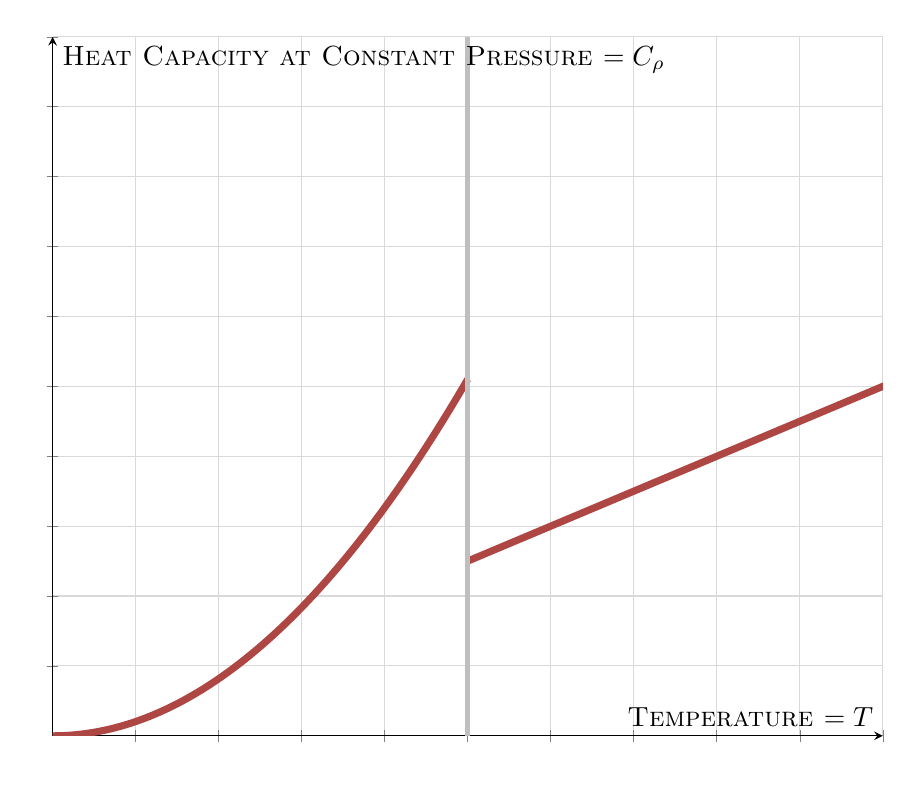
\begin{tikzpicture}
\begin{axis}[
width=\linewidth,
grid=major,
grid style={gray!30},
axis lines=middle,
xmax=10,
xmin=-0,
ymin=0,
ymax=1,
ylabel={\scshape Heat Capacity at Constant Pressure $=C_\rho$},
xlabel={\scshape Temperature $=T$},
xtick={},
xticklabels={},
ytick={},
yticklabels={},
restrict y to domain=-7:12
]

\addplot [redtea][line width=0.6ex,smooth,domain=5:30,samples=1000]{x/20};
\addplot [redtea][line width=0.6ex,domain=0:5,samples=1000]{pow(x/7,2)};
%\addplot [gray!50,line width=0.4ex]coordinates{(5,0)(5,30)};
\addplot+[
gray!50,line width=0.4ex,
mark=none,
const plot,
empty line=jump,
]
coordinates {
	(5,1)
	(5,-1)
};
\end{axis}
\end{tikzpicture}
\end{document}
